% Muscle description and static model

\chapter{Tap Water-Driven McKibben Artificial Muscle}
\label{ch:muscle}

McKibben muscles were invented by Joseph L. McKibben to motorize pneumatic art orthotics.
The structure of a McKibben artificial muscle consists
in general of an inner rubber tube enclosed into a braided outer sleeve,
usually made of nylon or other materials with similar properties.

Figure~\ref{fig:components} show the basic components that are used to
create a McKibben artificial muscle.

\begin{figure}[H]
	\centering
	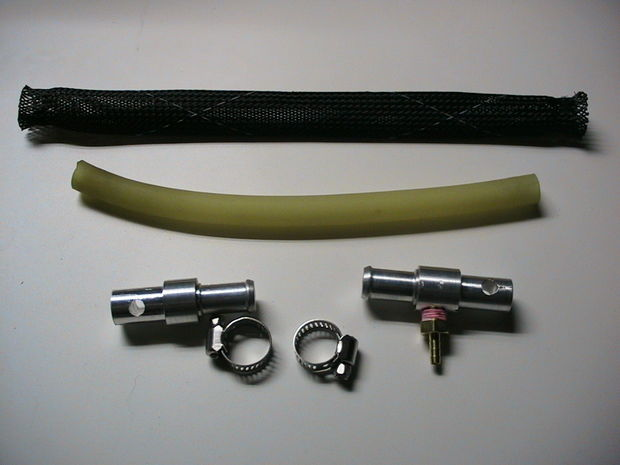
\includegraphics[width=.75\textwidth]{Images/muscle_components}
	\caption{McKibben artificial muscle basic components}
	\label{fig:components}
\end{figure}

This kind of muscle is almost exclusively pneumatic~\cite{chou1994static},
although research is increasing~\cite{kobayashi2017analysis} about the use of tap water for these actuators.
These muscles have relevant advantages with respect to conventional actuators. They:

\begin{itemize}
	\item have light weight;
	\item present a high power to weight ratio;
	\item possess high flexibility;
	\item have low cost;
	\item are environmentally friendly.
\end{itemize}

For these reasons, they are apt to be used as actuators for orthosis and prosthesis.
There are, however, some drawbacks: it is well known that the muscle
has poor control performance due to the existence of strong nonlinearities,
such as a hysteretic behaviour, as well as cavitation, by means of which
rapid changes of pressure in a liquid lead to the formation of small
vapor-filled cavities that implode, causing damage and instability,
and finally there may be problems due to saturation characteristics.
Furthermore, the wear of the materials composing the muscle, the nylon sleeve
and the rubber tube, may cause a shorter lifetime with respect to other actuators.

\begin{figure}[H]
	\centering
	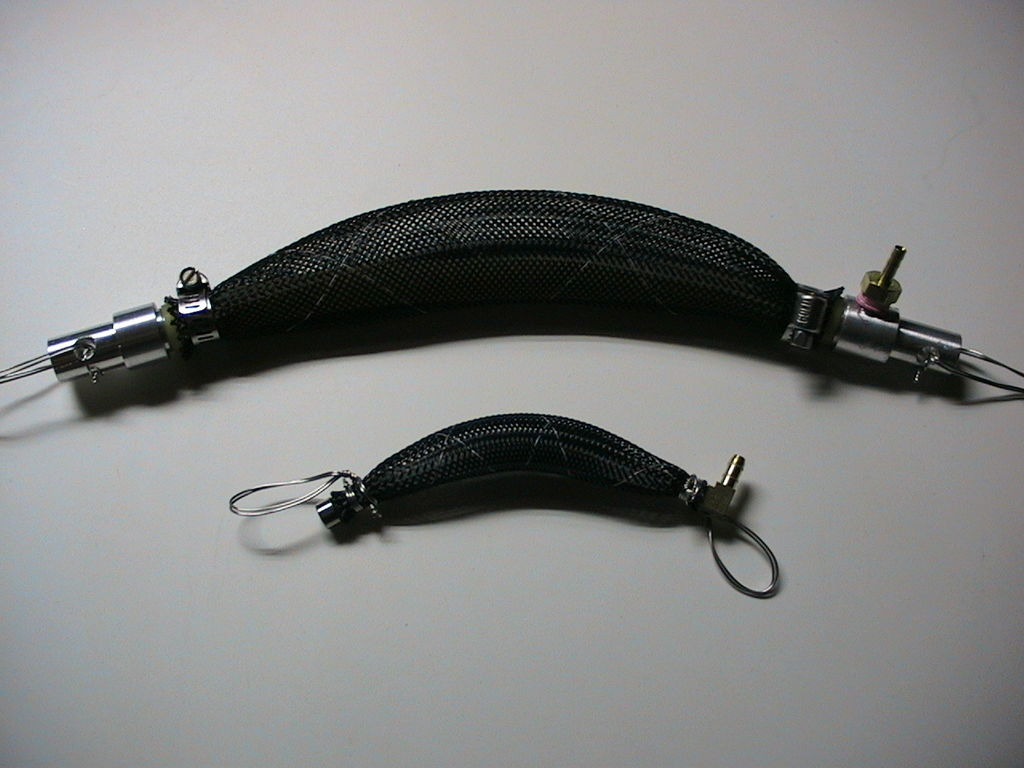
\includegraphics[width=.75\textwidth]{Images/muscle_complete}
	\caption{Operational McKibben artificial muscles}
	\label{fig:mckibben}
\end{figure}

Figure~\ref{fig:mckibben} shows operational braided McKibben
artificial muscles of different lengths.
























